\begin{frame}{Сравнение с монолитной детализацией}
    \begin{itemize}
        \item Сравнимое качество картинки (определяется на глаз)
        \item Метрики --- FPS и количество отправляемых на растеризацию треугольников
    \end{itemize}

    \begin{center}
        \begin{tabular}{lrrr}
            \hline \hline
            Тип отрисовки & FPS & Треугольников \\ \hline
            Наивысшее разрешение & 5.4 & 640 000 000 \\
            Монолитные лоды & \textbf{114.2} & 28 900 000 \\
            Кластерные лоды & 35.0 & 58 677 326 \\
            \hline \hline
        \end{tabular}
    \end{center}

    \alert{Производительность кластерных лодов пока недостаточна}
\end{frame}

\begin{frame}{Сравнение с монолитной детализацией}
    \begin{center}
        \begin{minipage}{.45\textwidth}
            \begin{center}
                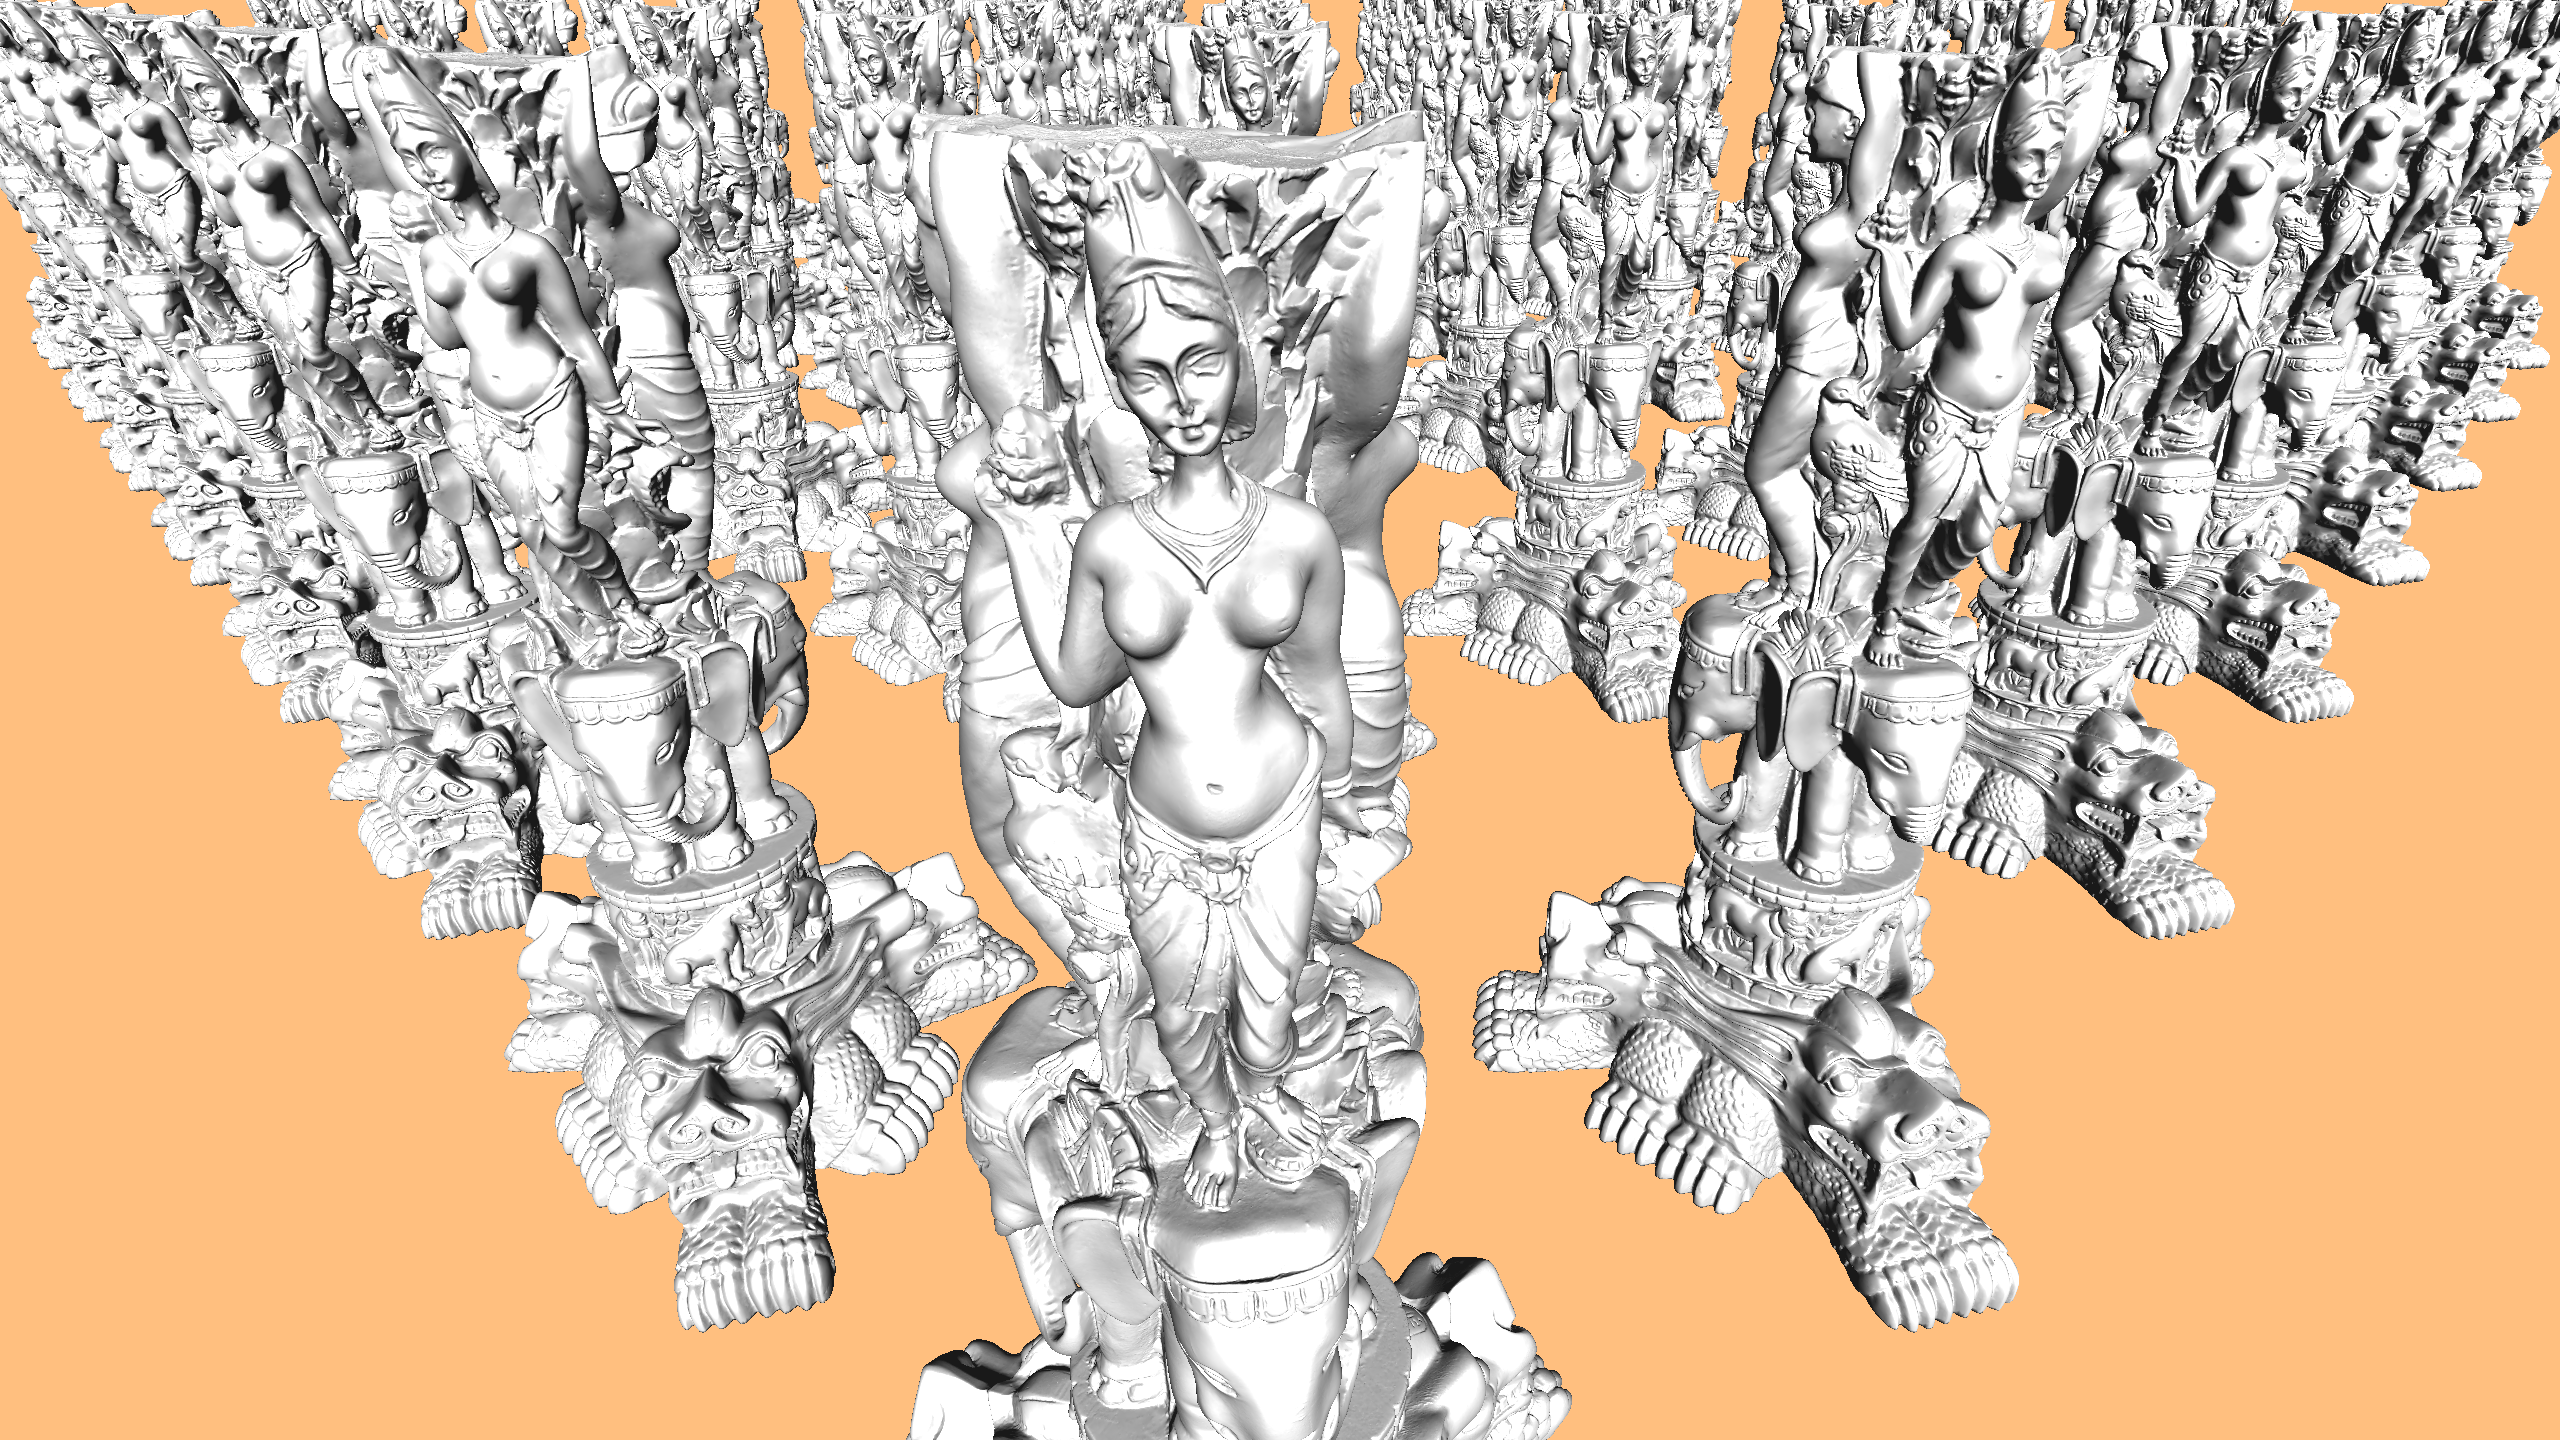
\includegraphics[width=\textwidth]{../Text/pics/comparison-mono.png}

                Монолитные лоды
            \end{center}
        \end{minipage}
        \begin{minipage}{.45\textwidth}
            \begin{center}
                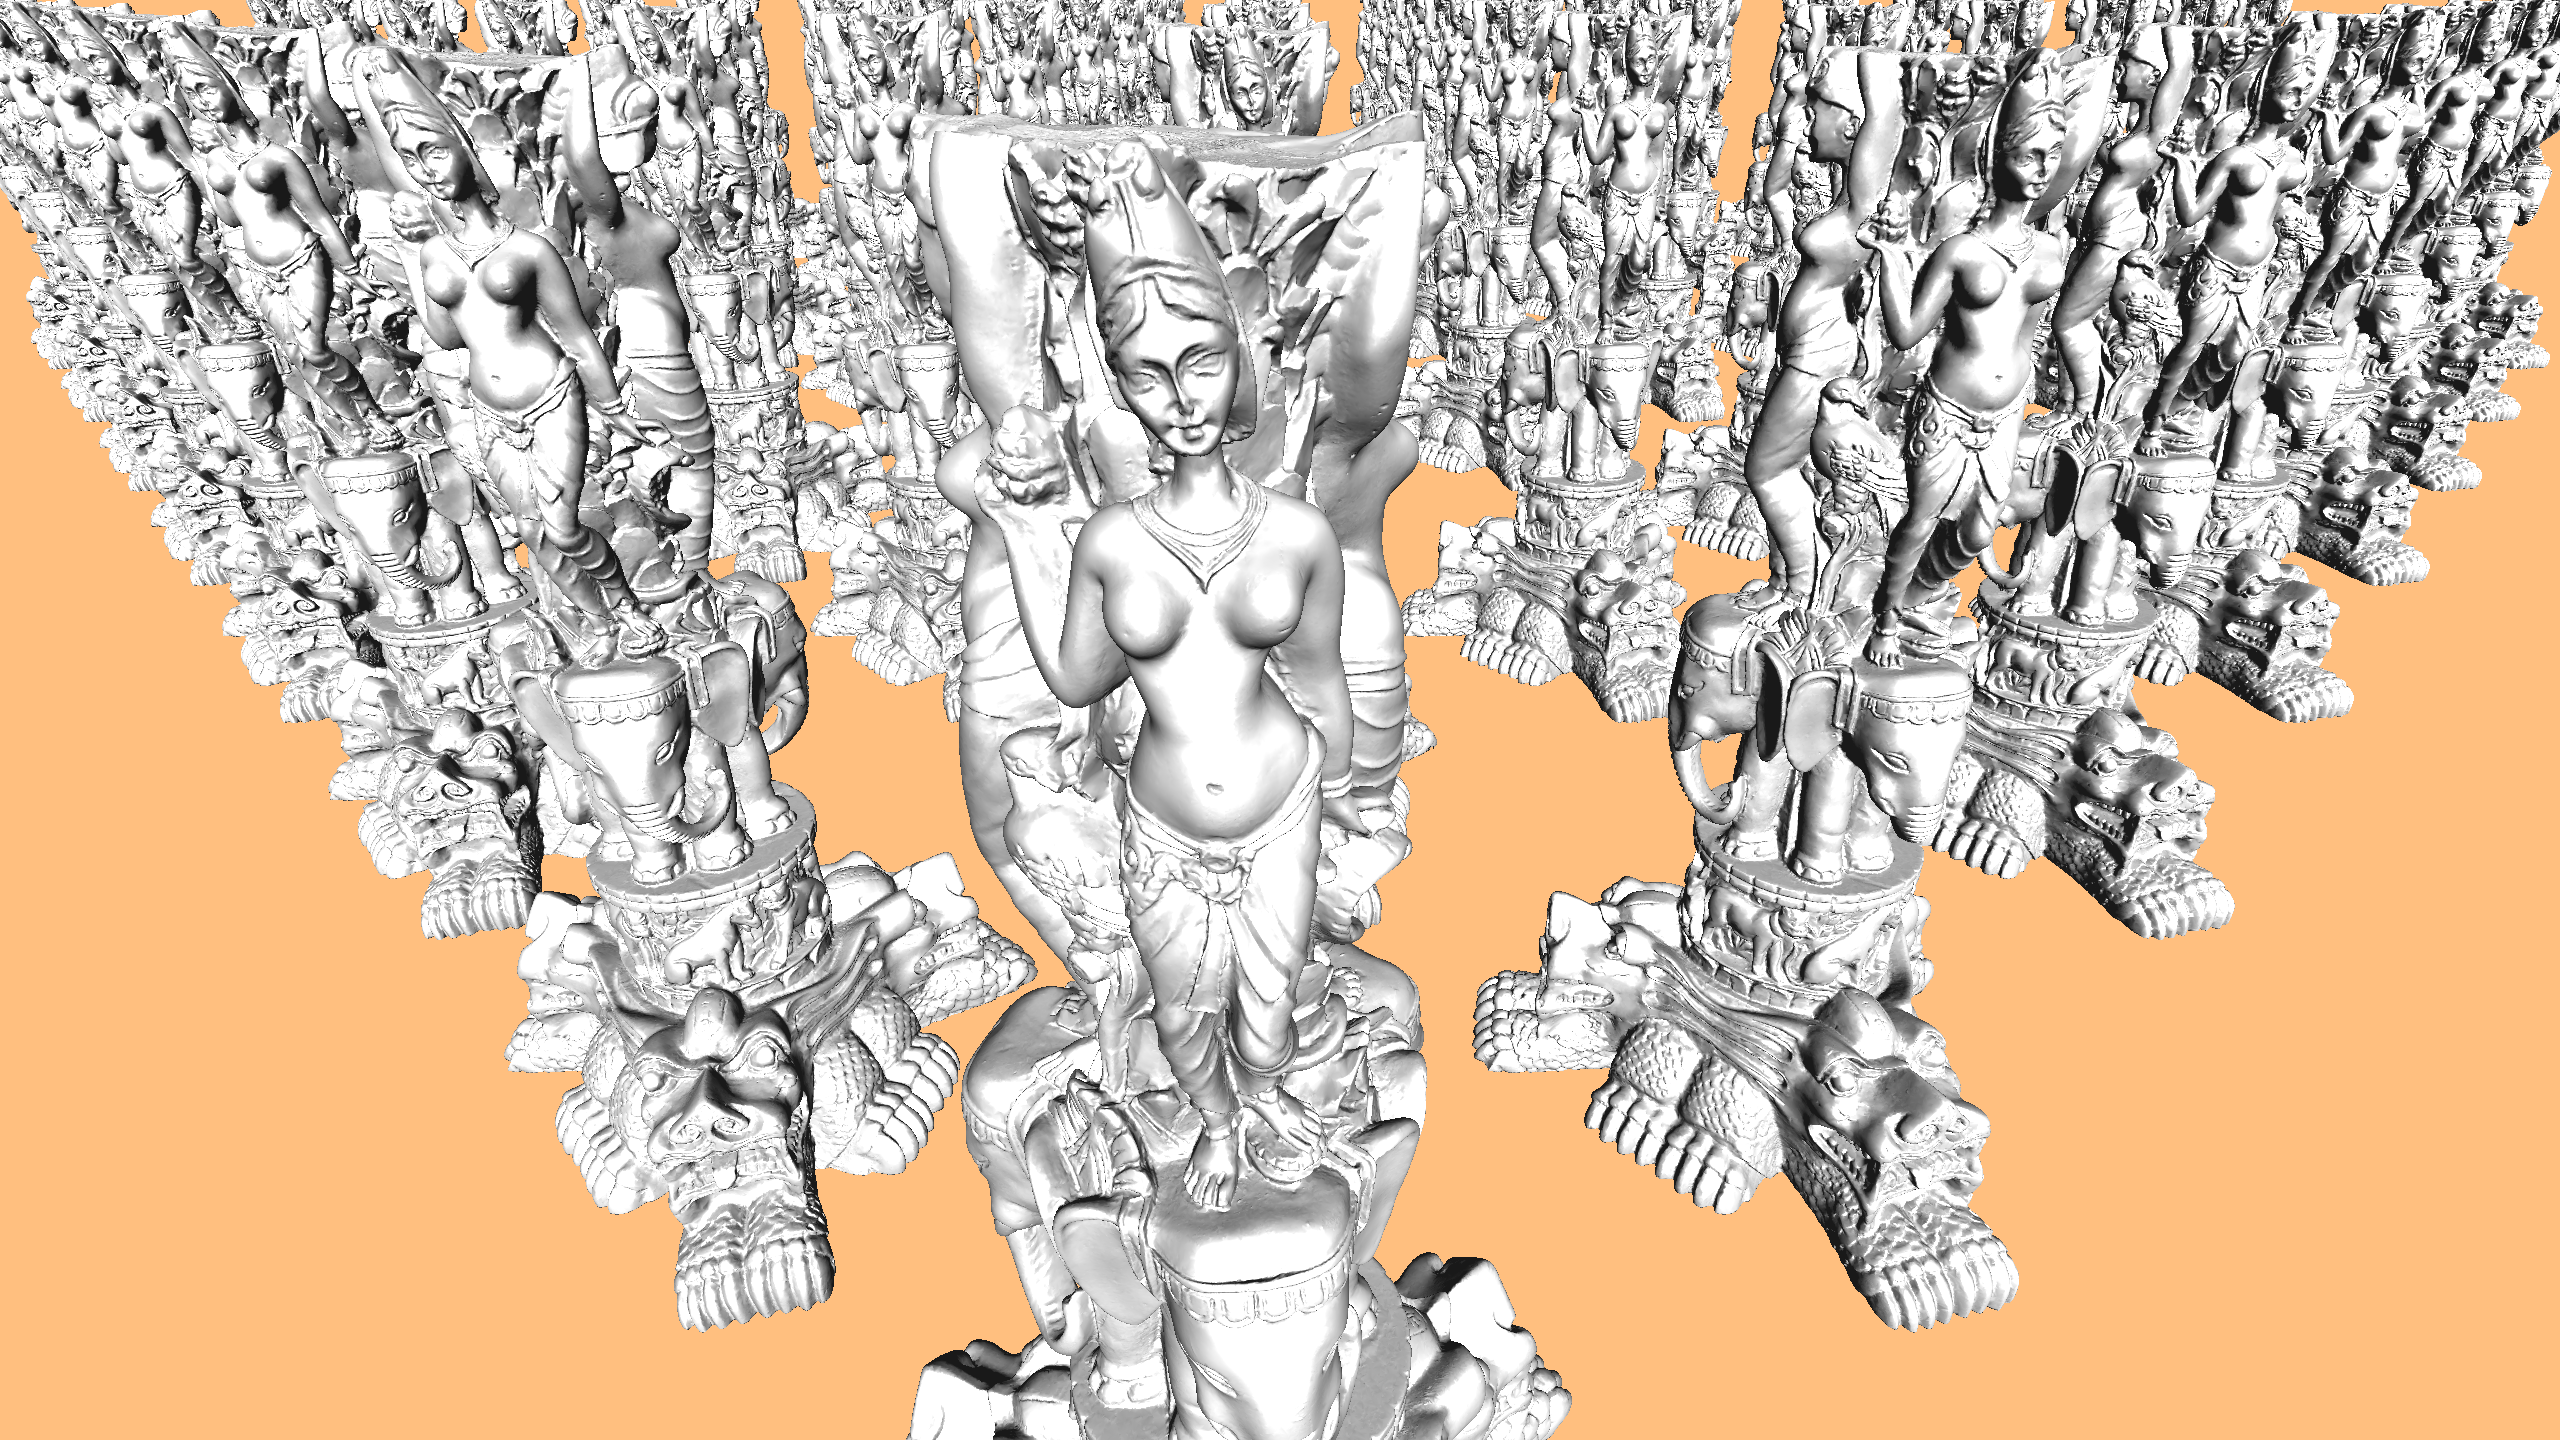
\includegraphics[width=\textwidth]{../Text/pics/comparison-cluster.png}

                Кластерные лоды
            \end{center}
        \end{minipage}
        \begin{minipage}{.45\textwidth}
            \begin{center}
                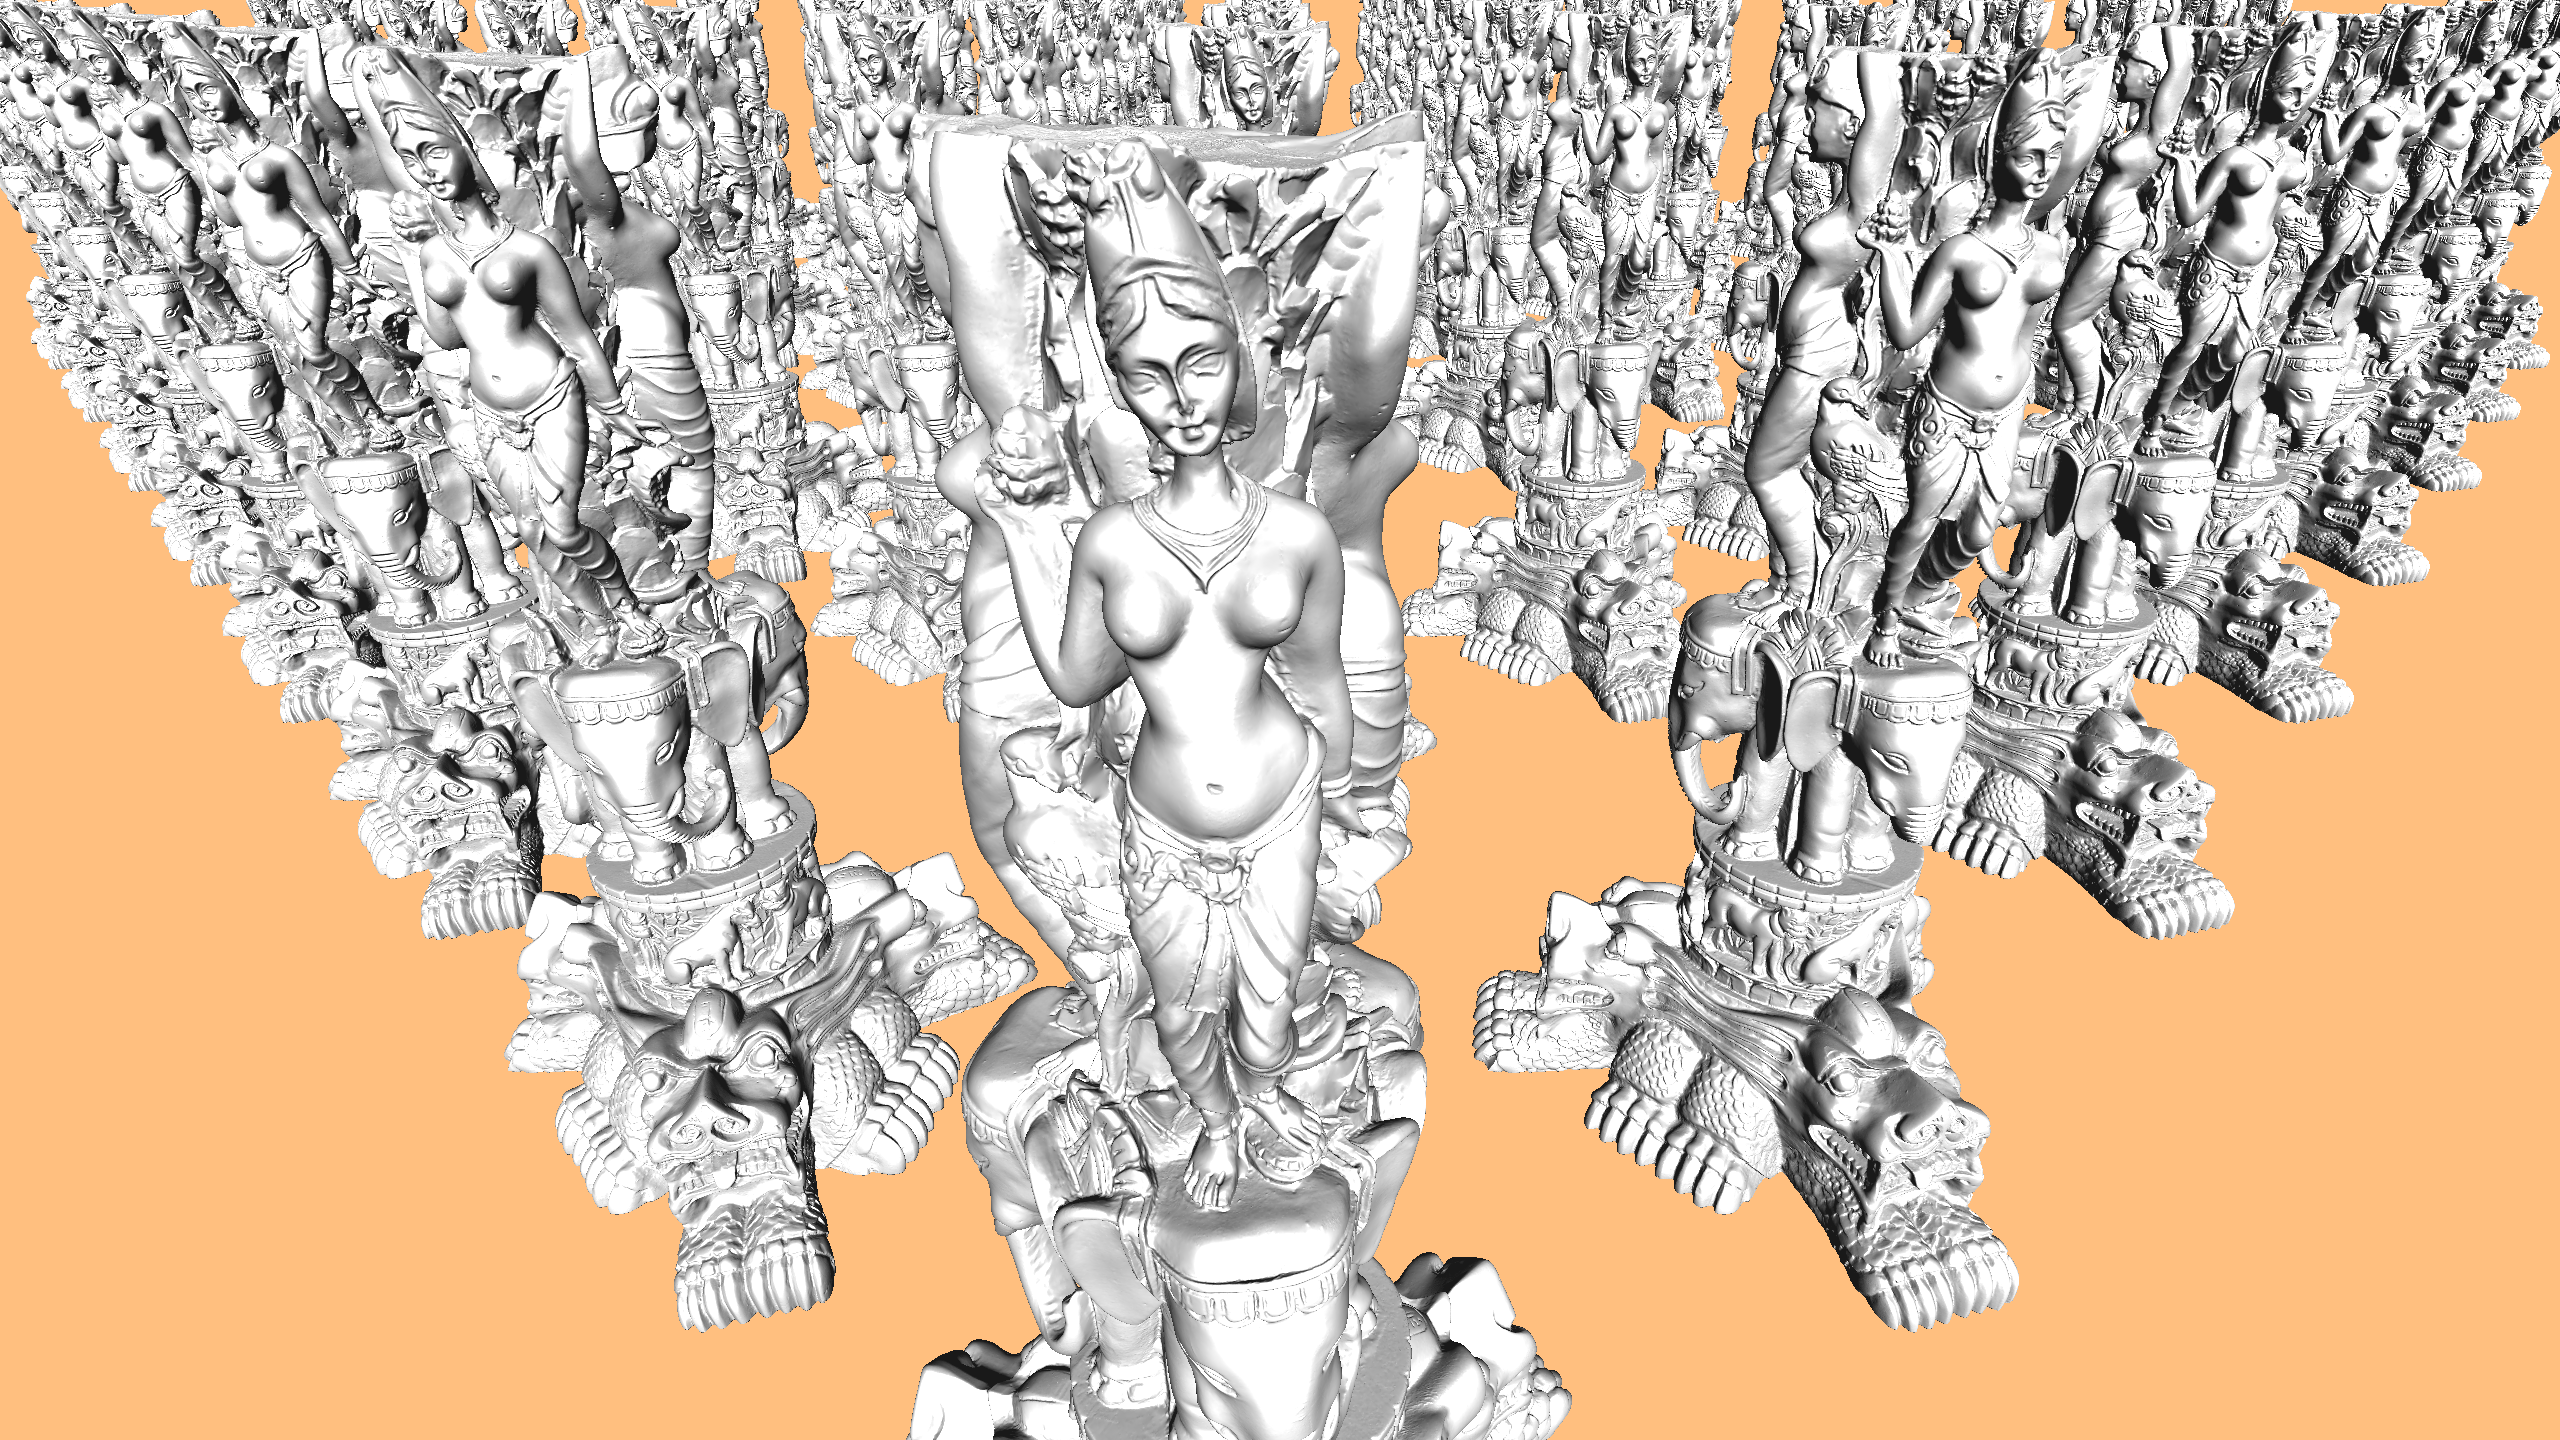
\includegraphics[width=\textwidth]{../Text/pics/comparison-0.png}

                Наивысшая детализация
            \end{center}
        \end{minipage}
    \end{center}
\end{frame}
